
%%%%%%%%%%%%%%%%%%%%%%%%%%%%%%%%%%%%%%%%%%%%%%%%%%%
    %Pakker og instillinger for dokumentet%
%%%%%%%%%%%%%%%%%%%%%%%%%%%%%%%%%%%%%%%%%%%%%%%%%%%

\documentclass[pdftex, 11pt, english, a4paper, twoside, parskip=full]{report} %%{article} 
\setcounter{secnumdepth}{4} % makes a number for \subsubsection

%\documentclass[pdftex, 10pt, english, a4paper, twoside, twocolumn]{article}

%\documentclass[5p,sort&compress]{elsarticle}		
% 5p gir 2 kolonner pr side. 1p gir 1 kolonne pr side.
% Valget sort&compress gjør at referansen [1,2,3] settes som [1-3]. 
% Andre innstillinger for "klassen" elsarticle finnes i dokumentasjonen på CTAN (http://www.ctan.org/pkg/elsarticle)

\usepackage{parskip}

\usepackage[margin=1in, tmargin=1.2in, bmargin=1.2in]{geometry}

\usepackage[english]{babel} %Legger til norske bokstaver

%\selectlanguage{norsk}%Får latex til å bruke norsk på steder der latex selv skriver ting. F.eks. Figur istedet for Figure	


\usepackage[T1]{fontenc} %Definerer hvilken font som skal brukes. For spesielt interesserte er dette en 8-bit encoding med fonter som bruker 256 glyfer
%\usepackage{times} %ev. charter er også en fin font :)
\usepackage{charter}
\renewcommand{\baselinestretch}{1.15} %fikser linjeavtstand %1.25 før 

\usepackage{pdfpages}

\usepackage[utf8]{inputenc}%Tillater deg å skrive norske bokstaver direkte fra tastaturet, i steden for å bruke kommandoer.		
\usepackage{graphicx, subcaption, ragged2e} % Nødvendig for å legge til bilder osv. 
% subcaption gjør at man kan dele opp figurer i a) og b) :D

%\usepackage{titleps} % for å lage top and bottom border :)

\usepackage[section]{placeins}
\usepackage{cancel}% for å kunne "stryke over" ting i ligninger feks \frac{\bcancel{b}}{\bcancel{b}} = 1
\usepackage{fmtcount}
\usepackage{siunitx} % Lar deg bruke kommandoene \SI{tall}{\enhet} og \si{\enhet}. feks \si{\milli\gram\per\liter}. Dette er en veldig fin måte for å få konsistene enheter på. 
\usepackage{booktabs}% lar deg bruke \toprule, \midrule og \bottomrule i tabeller for å lage pene tabeller.								
\usepackage{multirow}% Lar deg lage rader inni radene i en tabell.
\usepackage{listings}
%\usepackage[showframe=true]{geometry}
%\usepackage{changepage}????????

\usepackage{floatrow}% får flere figurer til å settes sammen
%\usepackage[document]{ragged2e}

\usepackage{setspace}
\usepackage{hyperref}
\hypersetup{
    colorlinks=true,
    linkcolor=blue,
    filecolor=blue,      
    urlcolor=blue,
    citecolor=black
    }
    
\usepackage{mfirstuc}

\usepackage{scrextend} % for å kunne referere til footnotes flere ganger i en tabell

\usepackage{rotating} %Gir deg en rekke muligheter for å rotere ting
\usepackage	{amsmath , amsfonts , amssymb}							
%\usepackage[hang,footnotesize,bf]{caption}% Gjør at captions under figurer og over tabeller blir pene.	

\usepackage[version=3]{mhchem} % Tillater deg å skrive kjemiske formler
\usepackage{epstopdf}% Omgjør .eps-filer til .pdf filer. Denne pakken er genial når man bruker chemdraw der man kan eksportere som eps. 
\usepackage{textcomp,gensymb}
\usepackage{float}% Tillater å bruke stor H i floats, dette kalles ofte for float of doom og er sjeldent anbefalt.

%\usepackage[super,square]{natbib}% Denne pakken er for bibliografien, super og square gjør at sitatet opphøyen og inlemmes av firkantparanteser. 

\usepackage{fancyhdr}% Lar deg lage den fine headeren på toppen av siden.
%\pagestyle{plain}
\pagestyle{fancy}

%\usepackage[Glenn]{fncychap}
%\ChRuleWidth{0.5pt}
%\ChTitleAsIs
%\ChTitleVar{\Huge\rm} %\rm = roman
%\ChTitleVar{\bfseries\Large\rm} %%% EXTRA
\usepackage[Lenny]{fncychap}
\ChNameVar{\fontsize{14}{16}\usefont{OT1}{phv}{m}{n}\selectfont}
\ChNumVar{\fontsize{60}{62}\usefont{OT1}{ptm}{m}{n}\selectfont}
\ChTitleVar{\Huge\bfseries\rm}
\ChRuleWidth{1pt}

\fancyhf[lh, rh, ch]{} 
\fancyhf[leh]{\leftmark} %lager header på venstre sida % nåværende chapter på venstre sida
\fancyhf[roh]{\rightmark} %lager header på høyre sida % nåværende section på høyre sida

%\fancyfoot{} 
%\fancyfoot[LE,RO]{\thepage} %%%%%%%%%%%%%%%%%%% FUNKER IKKE :/ Bare dropper det...
%\fancyfoot[LO,RE]{User Guide}

\usepackage{tikz}

\usepackage{siunitx}

\usepackage{appendix}

%\usepackage[style=apa , sorting=nyt]{biblatex}
\usepackage[style=authoryear, backend=bibtex]{biblatex}
%\usepackage{cite}
\addbibresource{references.bib} %navnet i krøllparantesene er navnet på .bib filen til bibliografien


%\usepackage[toc]{glossaries}

\usepackage{xcolor}
\usepackage{longtable}
\usepackage{pdfpages}

%%%%%%%%%%%%%%%%%%%%%%%%%%%%%%%%%%%%%%%%%%%%%%%%%%%%%%%%%%%%%%%%%%%%%%
%Setter noen instillinger for å gjøre ting pent :) 
\setlength\headheight{22.5pt}	
\floatstyle{plaintop}													
\restylefloat{table}													
\floatstyle{plain}														
\restylefloat{figure}													
\numberwithin{equation}{section}
\numberwithin{figure}{section}
\numberwithin{table}{section}

\raggedbottom %fikser rar spacing
%%%%%%%%%%%%%%%%%%%%%%%%%%%%%%%%%%%%%%%%%%%%%%%%%%%%%%%%%%%%%%%%%%%%%%

%Denne kodebiten lager en egen funksjon som heter \signature{}{} med input sted og navn. Den brukes litt lengre ned i koden
\newcommand{\signature}[2]{
\begin{minipage}[t]{0.9\textwidth}
\vspace{1cm}

    #1, \today
\vspace{1.5cm}

\setlength\parindent{0pt}
\begin{tabular}{cc}
    \rule{6cm}{1pt} & \hspace{2cm} \\
    #2 & 
\end{tabular}
\vspace{1cm}
\end{minipage}
}

% MAKING CHAPTER HEADER SMALLER
\usepackage{etoolbox}
\tracingpatches
\makeatletter
\newcommand{\makeCondensedChap}{%
\patchcmd{\@makeschapterhead}{\vspace*{50\p@}}{}{}{}%
\patchcmd{\@makeschapterhead}{\vskip 40\p@}{}{}{}%
}
%%%%%%%%%%%%%%%%%%%%%%%%%%%%%%%%%%%%%%%%%%%%%%%%%%%%%%%%%%%%%%%%%%%%%%

%\makeglossaries

%\newacronym{SPI}{SPI}{Soy Protein Isolate}

\begin{document}

%\pagenumbering{gobble}

\begin{titlepage} % Suppresses displaying the page number on the title page and the subsequent page counts as page 1
	\newcommand{\HRule}{\rule{\linewidth}{0.5mm}} % Defines a new command for horizontal lines, change thickness here
	
	\center % Centre everything on the page
	
	%------------------------------------------------
	%	Headings
	%------------------------------------------------
	
	\textsc{\LARGE IT3915 SPECIALIZATION PROJECT}\\[1.5cm] % Main heading such as the name of your university/college
	
	%\textsc{\Large NTNU}\\[1.5cm] % Major heading such as course name
	

	
	%------------------------------------------------
	%	Title
	%------------------------------------------------
	
	\HRule\\[0.4cm]
	
	{\huge\bfseries How can serious games inform about burnout in the workplace? (?)}\\[0.4cm] % Title of your document
	

	\HRule\\[1.5cm]
	

	%------------------------------------------------
	%	Author(s)
	%------------------------------------------------
	
	\begin{minipage}{0.4\textwidth}
		\begin{flushleft}
			\large
			\textit{Author}\\
			\textsc{Phajsi Choque Halvorsen\\} % Your name
		\end{flushleft}
	\end{minipage}
	~
	\begin{minipage}{0.4\textwidth}
		\begin{flushright}
			\large
			\textit{Supervisor}\\
			\textsc{Monica Divitini\\}
		\end{flushright}
	\end{minipage}
	
	
\vfill\vfill\vfill\vfill\vfill\vfill\vfill\vfill\vfill\vfill\vfill\vfill\vfill\vfill\vfill\vfill\vfill\vfill\vfill\vfill\vfill\vfill\vfill\vfill\vfill\vfill

	\begin{minipage}{\textwidth}
		\begin{figure}[H]
	    \centering
	    %\includegraphics[scale = 0.5]{Figurer/Estetisk/Maleri5.jpg}
	\end{figure}{}


	\begin{figure}[H]
	    \centering
	    %\includegraphics[scale = 1]{Figurer/Estetisk/NTNU-logo.PNG}
	\end{figure}{}
	
			
	\end{minipage}

	\vfill\vfill\vfill
	
	{\large\today}

	\vfill
	
\end{titlepage}
%
\pagenumbering{Roman}

\chapter*{Preface}
\addcontentsline{toc}{chapter}{Preface}


%
%\usepackage[margin=1in, tmargin=1.2in, bmargin=1.2in]{geometry}
%\newgeometry{textheight=28cm,voffset=-1cm,bottom=1cm}
%\newgeometry{textheight=28cm, left = 1cm, right = 1cm, bmargin=1.2in}
\newgeometry{textheight=27cm, left = 2.5cm, right = 2.5cm, bmargin=1.2in}

\chapter*{Abstract}
\markboth{}{}
\addcontentsline{toc}{chapter}{Abstract}

\vspace{-2cm}

\restoregeometry

%\input{Rapport/1-Abstract++/004 - Lists}
\tableofcontents

\chapter{Introduction}
\pagenumbering{arabic}


\section{Motivation}
Among the OECD member countries, Norway has the highest rate of employment for young people with higher education (25-34 years). The employment rate for this population is of 91\% for people with a bachelor's degree and 95\% for those with a master's degree \parencite{fazli_hoy_2022}. From this age, and until retirement this population will be working a considerable amount of years. Additionally, due to the rise of pension costs and living expectancy, the retirement age of about 67 years presently \parencite{noauthor_pensjonsalder_nodate} will likely increase. A retirement committee recently propositioned that the retirement age be increased regularly in the future \parencite{haugan_pensjonsutvalget_2022}.

With an expected employment duration of between 40 and 50 years for the present generation. It is a given that workplace well-being is primordial in living a good, healthy and happy life. Additionally, due to the recent pandemic and the stress it put on workers. An increase of the burnout rates has taken place around the globe. 

According to the Work and Well-being Survey of US adult workers by the \textit{American Psychological Association}, '3 in 5 employees reported negative impacts of work-related stress' in 2021 \parencite{abramson_burnout_2022}. In a survey done in Norway by \textit{Forskerforbundet} in 2021, 56\% of the respondents were not happy with the new working situation. The shift to teaching digitally, mixed with working from home added an increased workload. This added workload was reported by 40\% of the researchers, where only 16\% were compensated for it \parencite{svarstad_tarene_2021}. Similarly, in a longitudinal study carried out by \textit{Nasjonalt Kunnskapssenter om vold og traumatisk stress}, on hospital workers during the pandemic. They found that 20\% of the respondents reported significant anxiety and depression symptoms, and that one in six workers, about 16\%, reported burnout symptoms \parencite{noauthor_studie_2022}.

Not surprisingly, work movements like The Great Resignation and "quiet quitting" have arisen post-pandemic. A global increase in resignations is now known as The Great Resignation. The US reached a 20-year high "quit rate" in November 2021, where research by the \textit{Pew Reasearch Center} found that the main reasons for quitting was "low pay, a lack of opportunities for advancement and feeling disrespected at work" \parencite{parker_majority_2022}. Italy has seen an increase of 10\% in resignations in the middle of 2021, compared to 2019. Even quit rates in the tech-industry in India are at around 22\%, corresponding to a million of workers quitting at the end of 2021 \parencite{armillei_si_2021}. Another trend called "quiet quitting", started with TikTok. With "quiet quitting", workers are encouraged to prevent being overworked, instead achieving a greater work-life balance by only doing the job requirements, not going above and beyond \parencite{rosalsky_economics_2022}.

For all of these reasons, putting a spotlight on burnout; how it arises, how it can be prevented and how to get back from it, is important. Furthermore, enlightening the topic with the help of a serious game, will hopefully aid in preventing burnout, in an engaging and fun way.

\section{Context}
This project has been developed in collaboration with the Department of Computer Science at the Norwegian University of Science and Technology. The work is in foundation of an upcoming master thesis developing a serious game aiming to enlighten the workforce on burnout. 

\section{Research Questions}

As burnout can arise in a multitude of professions, to focus the research, this project will 

The research questions that this project will look into are the following:

\begin{itemize}
    \item[] \textbf{RQ1}: How can informative serious games be used to raise awareness around burnout in the IT profession?

To answer the research question, 
    \item[] \textbf{RQ1.1}: What kind of awareness about burnout do IT professionals have?
    \item[] \textbf{RQ1.2}: What type of burnout scenarios are relevant  for serious games?
\end{itemize}

\section{Results}

\section{Report Outline}
I think it will end up looking something like this
% TODO change at the end
\begin{itemize}
    \item introduction
    \item problem definition
    \item literature review (?)
    \item interviews
    \item discussion
    \item conclusion
\end{itemize}
\chapter{Problem Definition}  

% 1 - overview of the issue discussed in the paper, as well as its background and who it affects. It may also describe your objectives in performing your research. %Who acknowledges burnout officially - START
The \textit{World Health Organization}, WHO, added burnout to the \textit{International Classification of Diseases}, the ICD-11, in 2019. In it, burnout was defined as a syndrome resulting from "chronic workplace stress that has not been successfully managed" \parencite{who_notitle_2019}. 

% 2 - When research on burnout started - BACKGROUND
This recent addition was possible because of the research on burnout by Dr. Christina Maslach, the pioneer researcher on burnout. Burnout as a research field began in the 1970s, trying to make sense of the experience some workers got when they started a new job with enthusiasm and energy, only to over time end up disillusioned; and with feelings of exhaustion, frustration, anger and cynicism \parencite[38]{maslach_understanding_2017}.

\section{Three burnout dimensions}

From the initial research on the topic, common themes arrived that concluded with the three basic dimensions of the burnout experience: "an overwhelming exhaustion, feelings of cynicism and detachment from the job, and a sense of ineffectiveness and lack of accomplishment" %from (see Maslach, 1993). 
Maslach then developed the Maslach Burnout Inventory, together with a General Survey, to assess these three burnout dimensions in her research \parencite[38]{maslach_understanding_2017}.

Later, at the beginning og the twenty-first century, researchers have also looked into the opposite of burnout, identified as "engagement", but how exactly it relates to burnout is still debated \parencite[40]{maslach_understanding_2017}.

\textbf{Exhaustion}

Exhaustion reflects the strain dimension of burnout, the basic stress experienced by a person. It refers to the "feelings of being overextended and depleted of one’s emotional and physical resources" \parencite[41]{maslach_understanding_2017}. 

\textbf{Cynicism}

The cynicism dimension captures the individual's relationship to work, by assessing the negative, distancing response to their job and the people in it.

\textbf{Professional Inefficacy}

Exhaustion is not viewed as unprofessional, there can be pride associated to exhaustion. But exhaustion can prompt actions to distance oneself from work, most likely as a coping mechanism to work overload, leading to cynicism. Cynicism in contrast is viewed as unprofessional, and therefore these feelings are most likely not shared with others and they contribute to a diminished professional efficacy. 

When an individual experiences burnout with all its facets, they loose a "a psychological connection with their work that has implications for their motivation and their identity" \parencite[41]{maslach_understanding_2017}.

\section{Areas of Worklife Scale model}
The research on burnout has identified organizational risk factors across many occupations in various countries. Maslach and Leiter analyzed the research literature and identified six areas of worklife most relevant for the relationship that people develop with their work: workload, control, reward, community, fairness and values \parencite{brom_areas_2015}.

\textbf{Workload}\\
When job demands surpass human limits, the most likely consequence is emotional exhaustion. People doing too much in a short amount of time, with limited resources \parencites{brom_areas_2015}[44]{maslach_understanding_2017}.

\textbf{Control}\\
The control dimension includes the individual's perceived capacity to influence decisions related to their work, along with their ability to exercise personal autonomy and to access resources like social support, to complete their work \parencites{brom_areas_2015}.

\textbf{Rewards}\\
Rewards refers to the extent that workers perceive that rewards; both monetary, social and intrinsic rewards, are consistent with their personal expectations. If people feel they are neglected by the employer's material and social reward system, they will feel out of sync with its values \parencites{brom_areas_2015}.

\textbf{Community}\\
The community dimension assesses the overall quality of social interaction at work and the sense of community in an organization. It encompasses interpersonal conflicts, informal social support, closeness and the capacity to work as a team. Supervisor support is more consistently associated with exhaustion; reflecting the supervisors' impact on employees' workload, while coworker support is related to accomplishment or efficacy.
\parencites{brom_areas_2015}[46]{maslach_understanding_2017}.

\textbf{Fairness}\\
Fairness encompasses the extent to which decisions and resource allocation at work are perceived as fair \parencite{brom_areas_2015}

\textbf{Values}\\
Finally, the values dimension cover the ideals and motivation that appeal people to their jobs. They are therefore the motivating connection between the individual and the workplace. A value conflict in the job can be: that the worker makes a trade-off between work they want to do and work they do; that personal career aspirations or personal values are in conflict with the organizational values; or that the worker is caught between conflicting organizational values \parencites{brom_areas_2015}[47]{maslach_understanding_2017}.

% 3 - why burnout is important for the individual and workplaces - AFFECTS
\section{Outcomes of burnout}

Besides the negative burnout dimensions, the problem with burnout is it's role as a mediator of negative personal and professional outcomes.

\textbf{Work}

Burnout employees have greater job dissatisfaction, are less committed, more absent and are more intent to leave their jobs, which not surprisingly leads to poorer work performance. They have a negative effect on their colleagues, causing more personal conflicts and disrupting job tasks. These negative effects can "spill" over on workers' home life. Burnout workers were rated in more negative ways by their spouses. The workers themselves have reported that their work has impacted negatively their family and that their marriage was unsatisfactory \parencite[49]{maslach_understanding_2017}. 

\textbf{Health}

The exhaustion facet of burnout correlates to typical stress symptoms as headaches, chronic fatigue, gastrointestinal disorders, muscle tension, hypertension, cold and flu episodes, and sleep disturbances. A longitudinal study done by Maslach and Leiter, found that workload and exhaustion predicted the rate of workplace injuries during the following year. Other research has also found a link between burnout and lifestyle practices with health risks, like smoking, alcohol use and psychotropic drug use.  %(Leiter et al., 2013). 
In the mental health aspect, burnout is predictive of depression, anxiety and irritability \parencite[50]{maslach_understanding_2017}. %(Greenglass and Burke, 1990; Schonfeld, 1989) 
% Work outcomes Burnout has been frequently associated with various forms of negative
% responses to the job, including job dissatisfaction, low organizational commitment, absenteeism,
% intention to leave the job, and turnover (see Schaufeli and Enzmann, 1998, for a
% review). People who are experiencing burnout can have a negative impact on their colleagues,
% both by causing greater personal conflict and by disrupting job tasks. Thus, burnout can be
% “contagious” and perpetuate itself through social interactions on the job (Bakker, Le Blanc,
% and Schaufeli, 2005; Gonz´alez-Morales, Peir´o, Rodr´ıguez, and Bliese, 2012). Such findings
% suggest that burnout should be considered as a characteristic of workgroups rather than simply
% an individual syndrome.
% Burnout can also have a negative “spillover” effect on workers’ home life. Workers experiencing
% burnout were rated by their spouses in more negative ways (Jackson and Maslach,
% 1982; Zedeck, Maslach, Mosier, and Skitka, 1988), and they themselves reported that their
% work has a negative impact on their family and that their marriage is unsatisfactory (Burke
% and Greenglass, 1989; 2001).
\chapter{Literature Review?}

\section{Method}
\section{Results}
\section{Discussion}
%\chapter{Co-Design Workshop?}
*Read about participatory design and human-centered design

\section{Preparations}
\section{Workshop with participants}
\section{Discussion}
\chapter{Interviews with IT professionals (maybe?)}

\section{Purpose}
\section{Participants}
\section{Procedure}
\section{Results}
\section{Conclusion}
\section{Summary}
%\chapter{Discussion}
%\chapter{Conclusion}



\vfill % Gjør at signaturen havner nederst på siden, uavhengig av hvor mye tekst det er på den. Dette er en god praksis

%\twocolumn[
%\begin{@twocolumnfalse}

%\bibliographystyle{unsrtnat}%Definerer bibliografistil

%\addbibresource{bibliography.bib}



\printbibliography

%Vedleggene skal alltid komme etter referanselisten og skal plasseres i en egen fil, på en ny side. Derfor brukes \newpage
%\end{@twocolumnfalse}]

\addappendix

\newpage
%\cleardoublepage
\pagenumbering{Roman}
%%%%%%%%%%%%%%%%%%%%%%%%%%%%%%%%%%%%%%%%%%%%%%%%%%%%%%
\appendix
\chapter{Intervjumal}
\label{Intervjumal}
% 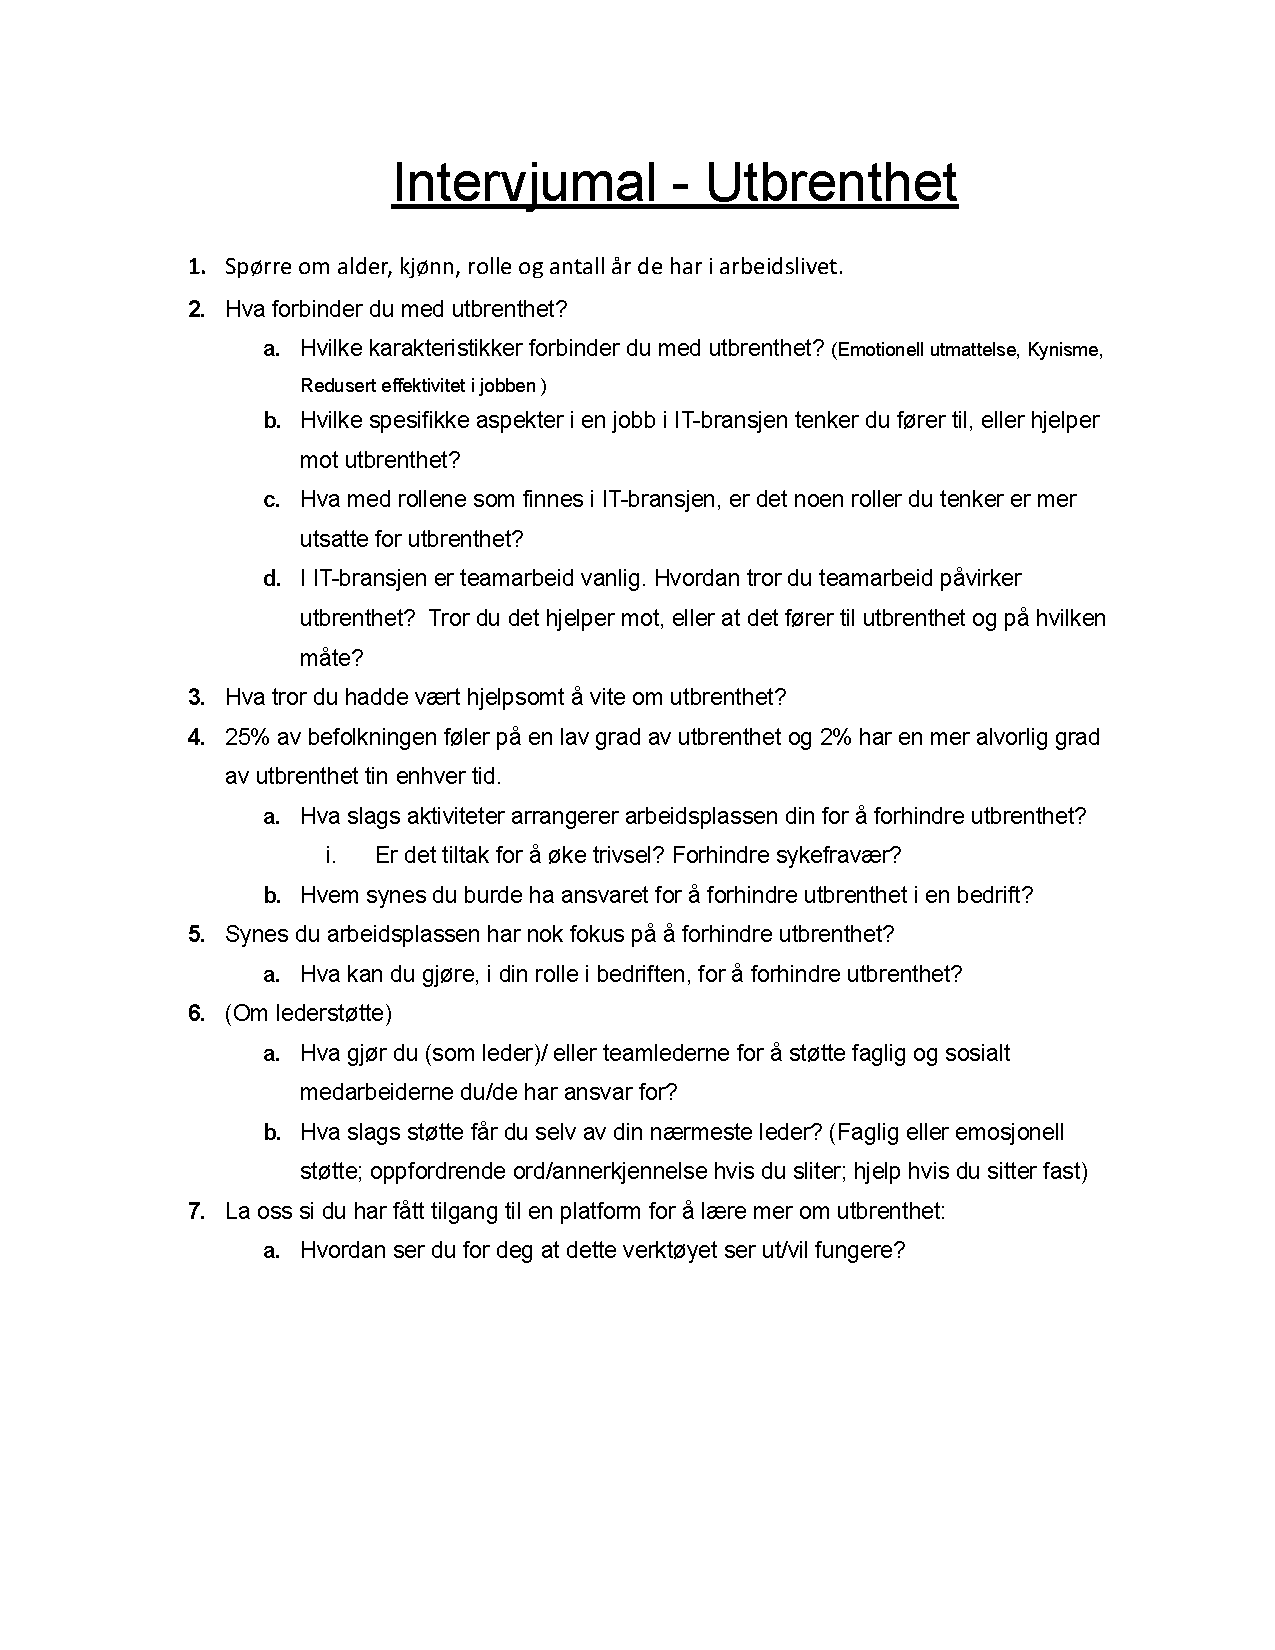
\includepdf[pages=1, 
%             fitpaper,
%             clip,
%             trim=3cm 6cm 2cm 4cm,
%             scale=0.5,
%             ]{Appendix/Intervjumal.pdf}
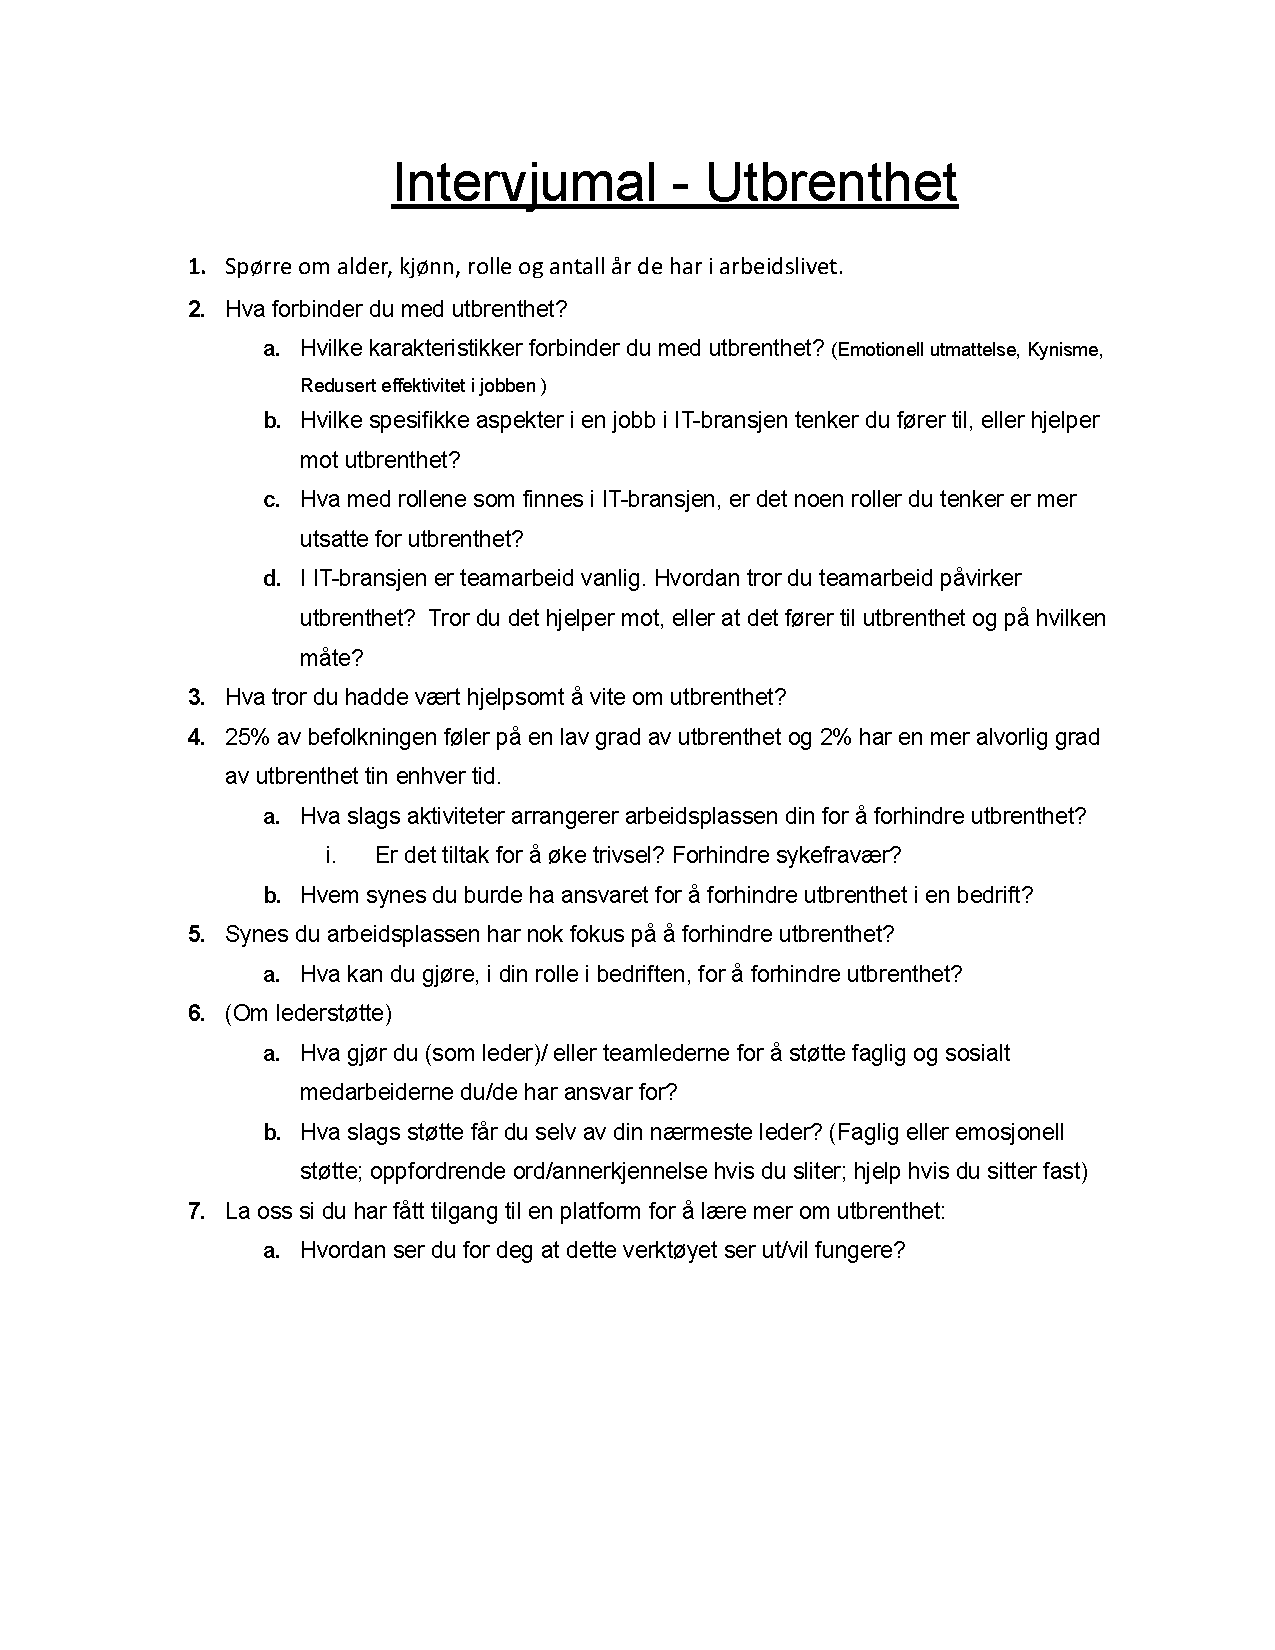
\includegraphics[
    page=1,
    clip,
    trim=3cm 6cm 2cm 4cm,
    keepaspectratio,
    scale=0.86,
]{Appendix/Intervjumal.pdf}
\noindent
\vfill














\newpage
\cleardoublepage

\end{document} 
